\section{I/O Processing Schemes}
\label{sec:io_processing}

This section presents a new zero-copy I/O processing scheme for GPU
computing. 
This scheme differs from the existing schemes in that both the GPU
execution and the data transfer times are minimized to meet a
requirement of low-latency GPU computing.
First of all, we introduce two existing schemes that are already
supported by CUDA.
We then present a new scheme, and also introduce a hybrid variant of our 
scheme and the existing one, which is suit for a specific case.

\subsection{Host and Device Memory ({\hd})}
\label{sec:hd}

\begin{figure}[!t]
 \centering
 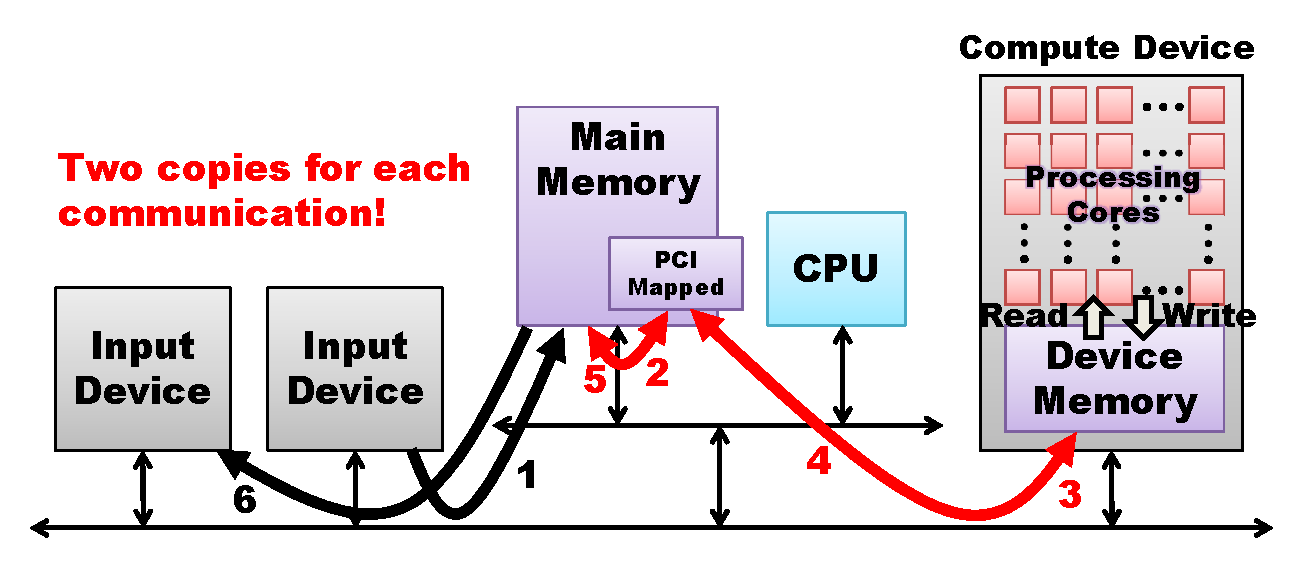
\includegraphics[width=\hsize]{eps/hd.eps}
 \caption{The traditional {\hd} scheme.}
 \label{fig:hd}
\end{figure}

This is the most common scheme of GPU computing in the literature.
In this scheme, there is space overhead in that the input and output
data must exist in both the device and the host memory at once.
Furthermore, there is a time penalty incurred to copy data, which is
almost proportional to the data size.
When applying this scheme, we allocate the same size of buffers to the
host and the device memory individually, and copy data between them
explicitly.

Figure~\ref{fig:hd} illustrates an overview of how this scheme works:
\begin{enumerate}
 \item The device driver of the input deivce configures the input device
       to send data to the allocated space of the host memory.
 \item The device driver of the GPU copies the data to the
       PCI-mapped space of the host memory, which is accessible to the
       device memory.
 \item The device driver of the GPU further copies the data to the
       allocated space of the device memory.
       Now, the GPU can access the data.
 \item When GPU computation is completed, the device driver of the
       GPU copies the output data back to the PCI-mapped space of the
       host memory.
 \item The device driver of the GPU further copies the output data back
       to the allocated space of the host memory.
 \item Finally, the device driver of the output device configures the
       output device to receive the data from the allocated space of the
       host memory.
\end{enumerate}

As desribed above, the {\hd} scheme incurs some overhead to copy the
same data twice for each direction of data transfer between the host and
the device memory.
This overhead might be a crucial penalty for low-latency GPU computing.

\subsection{Host Pinned Memory (Hpin)}

\begin{figure}[!t]
 \centering
 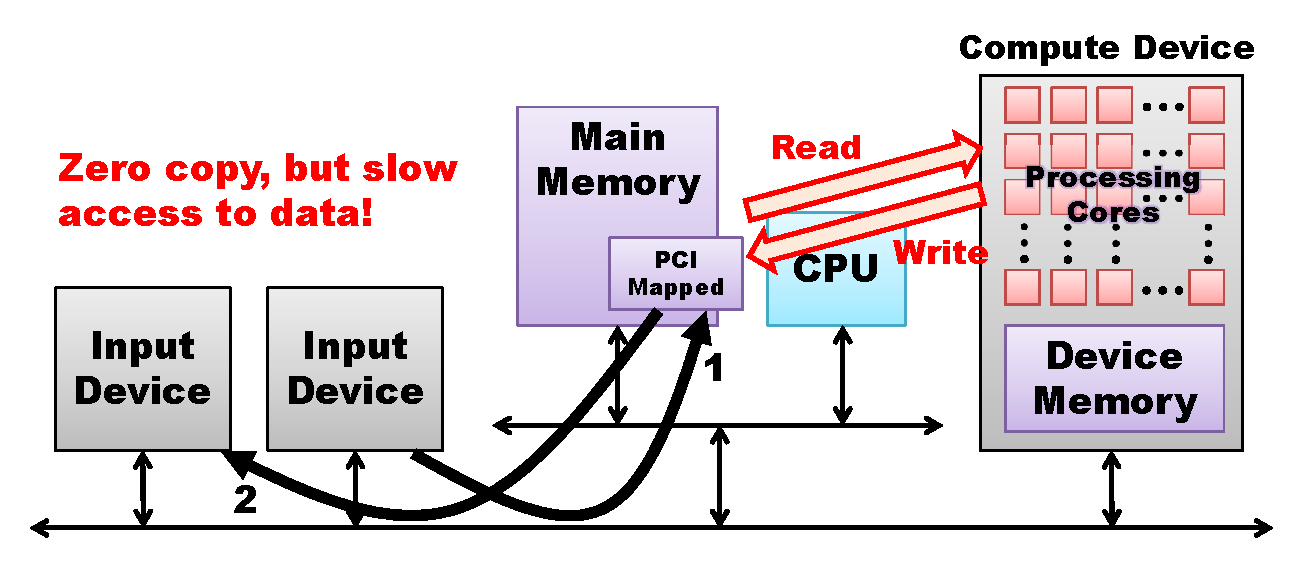
\includegraphics[width=\hsize]{eps/hp.eps}
 \caption{The zero-copy {\hp} scheme.}
 \label{fig:hp}
\end{figure}

As an alternative to allocating the buffers to both the host and the
device memory, we can allocate the buffers to page-locked PCI-mapped
space of the host memory, also known as \textit{pinned} host memory.
Since recent GPU architectures support unified addressing, this memory
space can be referenced by the GPU.
A major advantage of this scheme is that the input and the output
devices can also directly access this memory space, which means that
there is no need for intermediate buffers and data copies to have the
GPU access the data.

Figure~\ref{fig:hp} illustrates an overview of how this scheme works:

\subsection{Device Memory Mapped to Host (Dmap)}

\begin{figure}[!t]
 \centering
 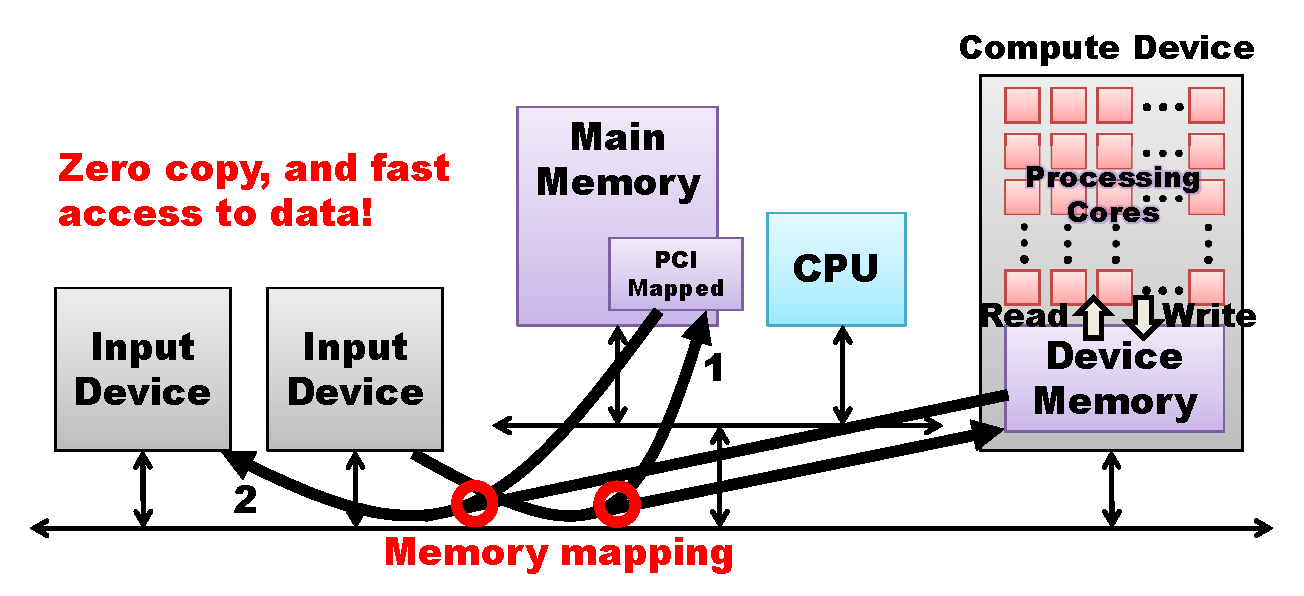
\includegraphics[width=\hsize]{eps/dm.eps}
 \caption{The zero-copy {\dm} scheme.}
 \label{fig:dm}
\end{figure}


The key to our method is having the host point directly to data on the GPU.
%We accomplish this by extending the CUDA API, adding the function {\tt cuMemMap()} which takes a pointer to already allocated space on the device
%and maps that space to a pointer declared on the host. 
This simplifies the programming paradigm in that no explicit copying needs
to take place -- the data can be referenced directly by the
host. This means that input data can be written directly to
the device without the need for intermediate buffers while the GPU
maintains the performance benefit of having the data on board.

This model is not limited to mapping GPU memory space to the host, it
is actually mapped to the PCI address space for the GPU which enables
other devices to access it. This is how direct communication
between the GPU and I/O devices is achieved.

\subsection{Device Memory Mapped Hybrid (DmapH)}
This method is the same as \dm\ as far as memory allocation and mapping. Like \dm\, the host references the GPU memory directly when writing data. For reading, however, we perform an explicit copy from GPU to host. The motivation for this is explained in our evaluation in section \ref{sec:evaluation}.

% merge with implementation
Although this memory mapping ability is used by NVIDIA's proprietary drivers it is not accessible to the programmer via the publicly available APIs (CUDA and OpenCL). To use this functionality our system requires the use of an open-source device driver such as nouveau or PathScale's pscnv\cite{ENZO}. 
%

